\documentclass{article}
\input{header}

\begin{document}
\rating{3}{2}

Let $G$ be a graph and $S \leq \operatorname{Aut}(G)$ be a subgroup of the automorphism group. We define a \emph{graph polyform} to be an induced subgraph of $G$ where two graph polyforms $p_1$ and $p_2$ are equivalent if there exists $s \in S$ such that the group action sends $s \cdot p_1 = p_2$.

If the $G$ is the infinite grid graph, and the automorphism group consists of all shifts and rotations of $G$, then the graph polyforms are the ``one-sided" polyominoes.

\begin{figure}[ht!]
  % \begin{tikzpicture}
  %   \node[circle, fill=red] (A1) at (0,0) {};
  %   \node[circle, fill=red] (A2) at (1,{sqrt(3)}) {};
  %   \node[circle, draw] (A3) at (2,0) {};
  %   \node[circle, draw] (A4) at (3,{sqrt(3)}) {};
  %   \node[circle, draw] (A5) at (4,0) {};
  %   \node[circle, draw] (A6) at (2,{2*sqrt(3)}) {};
  %   \draw[red,line width=0.1cm] (A1) edge (A2);
  %   \draw[line width=0.1cm] (A1) edge (A3);
  %   \draw[line width=0.1cm] (A2) edge (A3);
  %   \draw[line width=0.1cm] (A2) edge (A4);
  %   \draw[line width=0.1cm] (A3) edge (A4);
  %   \draw[line width=0.1cm] (A3) edge (A5);
  %   \draw[line width=0.1cm] (A4) edge (A5);
  %   \draw[line width=0.1cm] (A2) edge (A6);
  %   \draw[line width=0.1cm] (A4) edge (A6);
  % \end{tikzpicture}
  % \begin{tikzpicture}
  %   \node[circle, draw] (A1) at (0,0) {};
  %   \node[circle, fill=red] (A2) at (1,{sqrt(3)}) {};
  %   \node[circle, fill=red] (A3) at (2,0) {};
  %   \node[circle, draw] (A4) at (3,{sqrt(3)}) {};
  %   \node[circle, draw] (A5) at (4,0) {};
  %   \node[circle, draw] (A6) at (2,{2*sqrt(3)}) {};
  %   \draw[line width=0.1cm] (A1) edge (A2);
  %   \draw[line width=0.1cm] (A1) edge (A3);
  %   \draw[red, line width=0.1cm] (A2) edge (A3);
  %   \draw[line width=0.1cm] (A2) edge (A4);
  %   \draw[line width=0.1cm] (A3) edge (A4);
  %   \draw[line width=0.1cm] (A3) edge (A5);
  %   \draw[line width=0.1cm] (A4) edge (A5);
  %   \draw[line width=0.1cm] (A2) edge (A6);
  %   \draw[line width=0.1cm] (A4) edge (A6);
  % \end{tikzpicture}
   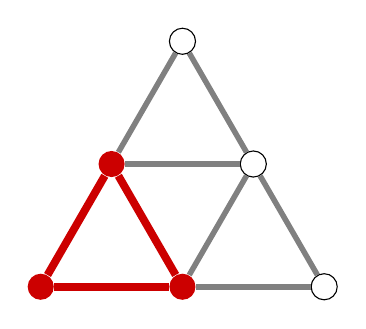
\begin{tikzpicture}[scale=0.9]
    \node[circle, fill=red!80!black] (A1) at (0,0) {};
    \node[circle, fill=red!80!black] (A2) at (1,{sqrt(3)}) {};
    \node[circle, fill=red!80!black] (A3) at (2,0) {};
    \node[circle, draw] (A4) at (3,{sqrt(3)}) {};
    \node[circle, draw] (A5) at (4,0) {};
    \node[circle, draw] (A6) at (2,{2*sqrt(3)}) {};
    \draw[red!80!black,line width=0.1cm] (A1) edge (A2);
    \draw[red!80!black, line width=0.1cm] (A1) edge (A3);
    \draw[red!80!black, line width=0.1cm] (A2) edge (A3);
    \draw[gray, line width=0.07cm] (A2) edge (A4);
    \draw[gray, line width=0.07cm] (A3) edge (A4);
    \draw[gray, line width=0.07cm] (A3) edge (A5);
    \draw[gray, line width=0.07cm] (A4) edge (A5);
    \draw[gray, line width=0.07cm] (A2) edge (A6);
    \draw[gray, line width=0.07cm] (A4) edge (A6);
  \end{tikzpicture}
  \hfill
  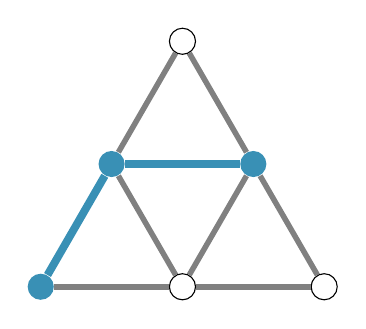
\begin{tikzpicture}[scale=0.9]
    \node[circle, fill=cyan!70!black] (A1) at (0,0) {};
    \node[circle, fill=cyan!70!black] (A2) at (1,{sqrt(3)}) {};
    \node[circle, draw] (A3) at (2,0) {};
    \node[circle, fill=cyan!70!black] (A4) at (3,{sqrt(3)}) {};
    \node[circle, draw] (A5) at (4,0) {};
    \node[circle, draw] (A6) at (2,{2*sqrt(3)}) {};
    \draw[cyan!70!black,line width=0.1cm] (A1) edge (A2);
    \draw[gray, line width=0.07cm] (A1) edge (A3);
    \draw[gray, line width=0.07cm] (A2) edge (A3);
    \draw[cyan!70!black,line width=0.1cm] (A2) edge (A4);
    \draw[gray, line width=0.07cm] (A3) edge (A4);
    \draw[gray, line width=0.07cm] (A3) edge (A5);
    \draw[gray, line width=0.07cm] (A4) edge (A5);
    \draw[gray, line width=0.07cm] (A2) edge (A6);
    \draw[gray, line width=0.07cm] (A4) edge (A6);
  \end{tikzpicture}
  \hfill
  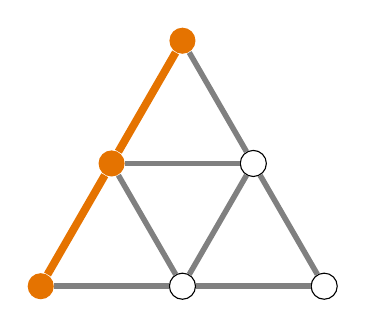
\begin{tikzpicture}[scale=0.9]
    \node[circle, fill=orange!90!black] (A1) at (0,0) {};
    \node[circle, fill=orange!90!black] (A2) at (1,{sqrt(3)}) {};
    \node[circle, draw] (A3) at (2,0) {};
    \node[circle, draw] (A4) at (3,{sqrt(3)}) {};
    \node[circle, draw] (A5) at (4,0) {};
    \node[circle, fill=orange!90!black] (A6) at (2,{2*sqrt(3)}) {};
    \draw[orange!90!black,line width=0.1cm] (A1) edge (A2);
    \draw[gray, line width=0.07cm] (A1) edge (A3);
    \draw[gray, line width=0.07cm] (A2) edge (A3);
    \draw[gray, line width=0.07cm] (A2) edge (A4);
    \draw[gray, line width=0.07cm] (A3) edge (A4);
    \draw[gray, line width=0.07cm] (A3) edge (A5);
    \draw[gray, line width=0.07cm] (A4) edge (A5);
    \draw[orange!90!black,line width=0.1cm] (A2) edge (A6);
    \draw[gray, line width=0.07cm] (A4) edge (A6);
  \end{tikzpicture}
  \hfill
  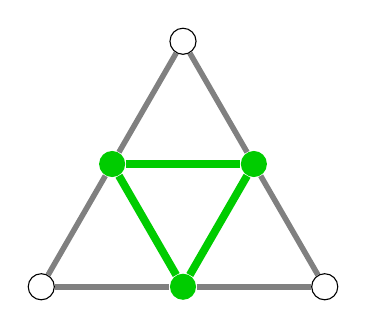
\begin{tikzpicture}[scale=0.9]
    \node[circle, draw] (A1) at (0,0) {};
    \node[circle, fill=green!80!black] (A2) at (1,{sqrt(3)}) {};
    \node[circle, fill=green!80!black] (A3) at (2,0) {};
    \node[circle, fill=green!80!black] (A4) at (3,{sqrt(3)}) {};
    \node[circle, draw] (A5) at (4,0) {};
    \node[circle, draw] (A6) at (2,{2*sqrt(3)}) {};
    \draw[gray, line width=0.07cm] (A1) edge (A2);
    \draw[gray, line width=0.07cm] (A1) edge (A3);
    \draw[green!80!black, line width=0.1cm] (A2) edge (A3);
    \draw[green!80!black, line width=0.1cm] (A2) edge (A4);
    \draw[green!80!black, line width=0.1cm] (A3) edge (A4);
    \draw[gray, line width=0.07cm] (A3) edge (A5);
    \draw[gray, line width=0.07cm] (A4) edge (A5);
    \draw[gray, line width=0.07cm] (A2) edge (A6);
    \draw[gray, line width=0.07cm] (A4) edge (A6);
  \end{tikzpicture}
  \caption{
    The four $3$-vertex graph forms of the triforce graph, up to the six isomorphisms of the graph.
    There is
    $1$ $0$-vertex form,
    $2$ $1$-vertex forms,
    $2$ $2$-vertex forms,
    $4$ $3$-vertex forms,
    $3$ $4$-vertex forms,
    $2$ $5$-vertex forms, and
    $1$ $6$-vertex form.
  }
\end{figure}

\begin{question}
  Suppose $G$ is a graph of order $n$. When does there exist some $k$ such that the graph polyforms of size $k$ partition $n$?
\end{question}

\begin{related}
  \item Let $f_G(k)$ be the number of graph polyforms of size $k$. When does this sequence fail to be unimodal?
  \item Which graphs of order $n$ admit the most graph polyforms of any size?
  % These need to have a lot of edges, but not a lot of automorphisms.
\end{related}

\end{document}
